\section{Tensions in the Cosmological Model} \label{sec:tensions}

The previous sections served to introduce and demonstrate the power of the $\Lambda$CDM model in describing the Universe. Nonetheless, tensions have emerged 
between cosmological parameter measurements obtained from different probes, suggesting that the discrepancies may be of physical or systematic origin. 
Here we present the three main tensions. \\

\subsection{$H_0$ Tension}

The Hubble constant $H_0$ can be inferred in two ways: through direct measurements via the cosmic distance ladder, or indirectly through model-dependent fitting of 
early-Universe observables. The direct measurement is obtained by calibrating standard candles such as Cepheid variables and Type Ia supernovae. 
Results from the SH0ES collaboration give $H_0 = 73.04 \pm 1.04\,\text{km}\,s^{-1}\,\text{Mpc}^{-1}$ (\cite{Riess_2022}). The indirect method relies on fitting the acoustic peak 
structure of the CMB angular power spectrum within the $\Lambda$CDM framework. The Planck 2018 collaboration reports $H_0 = 67.4 \pm 0.5\,\text{km}\,s^{-1}\,\text{Mpc}^{-1}$ 
(\cite{Planck_2018_params}), yielding a $\sim 5\sigma$ discrepancy with the SH0ES result. We see this in Figure \ref{fig:h0_tension}. This tension persists across multiple independent measurements of $H_0$ 
(\cite{DiValentino_2021}), raising the question of whether it reflects unknown systematic errors, or new physics beyond $\Lambda$CDM present at different 
epochs of the Universe. Recent results from the Chicago-Carnegie Hubble Program (CCHP) (\cite{Freedman_2025}) have measured the $H_0$ value using independent data from the James Webb Space Telescope 
with three independent methods (Tip of the Red Giant Branch (TRGB), J-Region Asymptotic Giant Branch (JAGB) and Cepheids). Their results show that with TRGB and 
JAGB the $H_0$ values are compatible with Planck measurements indicating that the tension arises from systematic effects. Moreover, a recent study by \cite{Stiskalek_2025} explicitly accounted 
for peculiar velocities when measuring $H_0$ using the same data as the one used in SH0ES and obtained a smaller value than the one reported by SH0ES of $H_0 = 71.1\pm 1.4 \, \text{km}\,s^{-1}\,\text{Mpc}^{-1}$ highlighting the importance of modeling peculiar velocities. 
The paper also highlights that whether the sample selection is done on supernova magnitude or host galaxy redshift does not significantly impact the value of $H_0$. 
Figure \ref{fig:h0_tension} shows $H_0$ measurements from different probes, highlighting the tension. \\

\begin{figure}[ht]
    \centering
    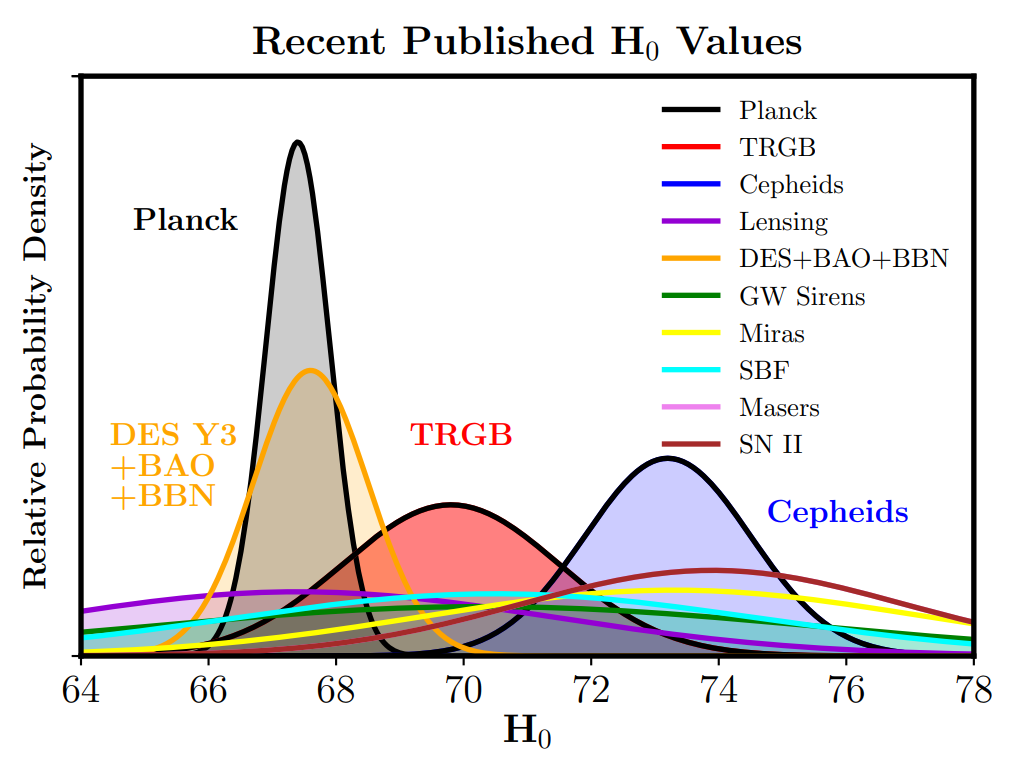
\includegraphics[width=0.8\textwidth]{MainLayout/Introduction_chapter/figures/h0_tension.png}
    \caption{Probability density functions of $H_0$ from different measurements probed at different redshifts, taken from \cite{Freedman_2021}. The CMB measurements prefer a lower $H_0$ value while Cepheids prefer higher values.}
    \label{fig:h0_tension}
\end{figure}

\subsection{$S_8$ Tension}

The parameter $S_8 = \sigma_8\sqrt{\Omega_m/0.3}$ combines the amplitude of matter fluctuations $\sigma_8$ with the matter density $\Omega_m$, and 
characterises the growth of large-scale structure. It can be measured both through the spatial correlations of galaxies and weak gravitational lensing, and through 
the CMB anisotropy power spectrum, where it is related to the primordial amplitude $A_s$ through the linear growth of structure. The Planck 2018 collaboration 
measures $S_8 = 0.832 \pm 0.013$ (\cite{Planck_2018_params}), while the Dark Energy Survey Year 6 measures $S_8 = 0.789^{+0.012}_{-0.012}$ from a combination 
of cosmic shear, galaxy clustering, and galaxy-galaxy lensing (\cite{DES_y6}), indicating a $2.3\sigma$ discrepancy (Figure \ref{fig:s8_tension}). \\

\begin{figure}[ht]
    \centering
    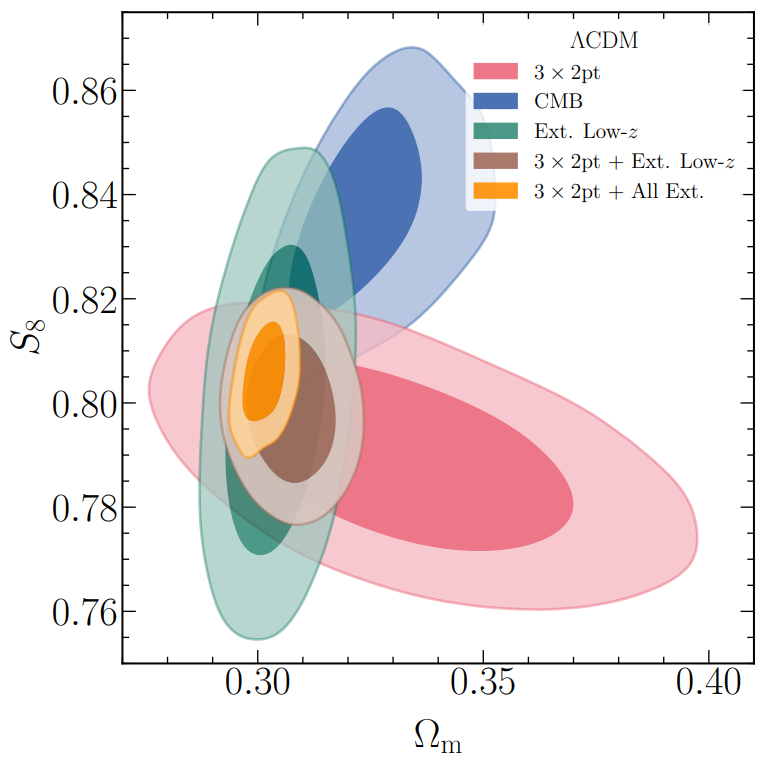
\includegraphics[width=0.8\textwidth]{MainLayout/Introduction_chapter/figures/s8_tension_des.png}
    \caption{$S_8$ and $\Omega_m$ contours for different galaxy surveys and CMB taken from \cite{DES_y6} enclosing the 68\% and 95\% posterior probability. The combination of the DES results with all of the other probes is in orange while the CMB measurements are in blue.}
    \label{fig:s8_tension}
\end{figure}

\subsection{$(w_0, w_a)$ Tension}

Within the $\Lambda$CDM paradigm, the accelerated expansion of the Universe is driven by a cosmological constant with equation of state $w = -1$, corresponding 
to a constant dark energy density $\rho_\Lambda = \text{const}$. If instead the dark energy density evolves with time, the simplest extension is the 
Chevallier-Polarski-Linder (CPL) parametrisation (\cite{Chevallier_2001}, \cite{Linder_2003}): 
\begin{equation}
    w(a) = w_0 + w_a(1-a)
\end{equation}
where $w_0$ is the present-day equation of state and $w_a$ parametrises its time evolution. The $\Lambda$CDM limit is recovered for $w_0 = -1$ and $w_a = 0$. \\

Recent results from DESI DR2, when combined with Planck CMB data and Type Ia supernova datasets, show deviations from $\Lambda$CDM in the $(w_0, w_a)$ plane 
(\cite{DESI_DR2_2025}). The significance of the deviation depends on the supernova sample used: $2.8\sigma$ when combined with Pantheon+, $3.8\sigma$ with 
Union3, and $4.2\sigma$ with DES Year 5 (Figure \ref{fig:w0_tension}) (\cite{DESI_DR2_2025}). A subsequent recalibration of the DES Year 5 supernova sample (DES-SN5YR, \cite{Popovic_2025}) reduced 
this DES discrepancy to $3.2\sigma$. \\

\begin{figure}[ht]
    \centering
    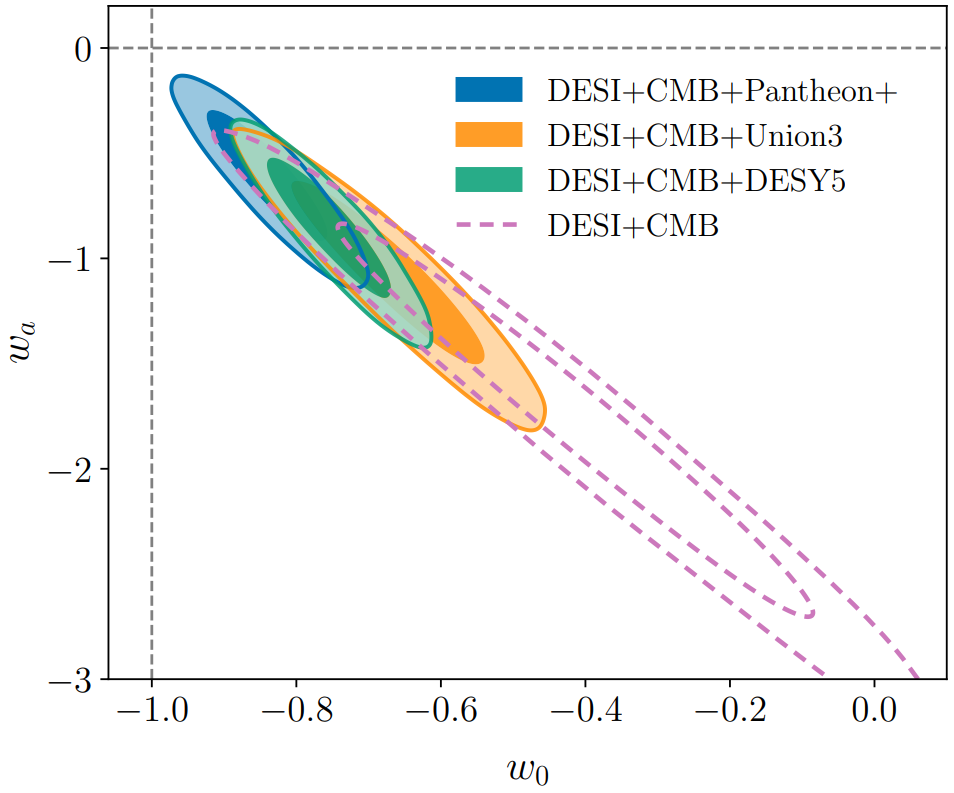
\includegraphics[width=0.8\textwidth]{MainLayout/Introduction_chapter/figures/w0_wa_tension.png}
    \caption{$w_0$ and $w_a$ contours from the latest \cite{DESI_DR2_2025} measurements enclosing the 68\% and 95\% posterior probability when 
    combined with Pantheon+ (blue), Union3 (orange) and DES-SN5YR (green) and CMB (purple dotted lines). }
    \label{fig:w0_tension}
\end{figure}